\documentclass[a4paper]{scrartcl}


\usepackage[utf8]{inputenc}
\usepackage[ngerman]{babel}
\usepackage{enumerate}
\usepackage{tikz}
\usepackage{fancyhdr}
\usepackage{lastpage}
\usepackage{verbatim}

\usepackage{listings}
\setlength{\parindent}{0mm}
\usepackage{graphicx}
\usepackage{amsmath}
\usepackage{algorithm2e}

\pagestyle{fancy}
\fancyhead[L]{Wintersemester\\2016/2017}
\fancyhead[C]{Enterprise Computing Praktikum\\Blatt 4}
\fancyhead[R]{Nikolas Zeitler\\Joshua Hartmann}

\fancyfoot[L]{}
\fancyfoot[C]{\thepage /\pageref{LastPage}}
\fancyfoot[R]{}

\renewcommand{\textheight}{700px}
\renewcommand{\footskip}{10px}
\newcommand*\xor{\mathbin{\oplus}}
\begin{document}
	\section{Aufgabe}
	\subsection{Screenshot von SELECT}
	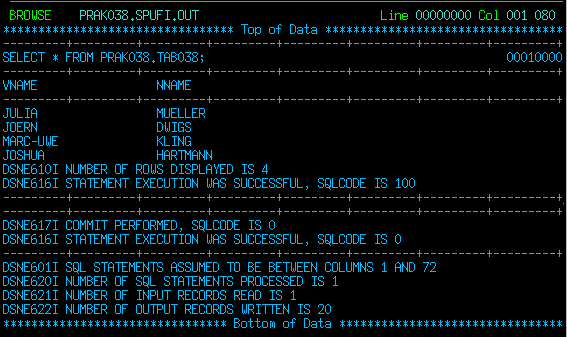
\includegraphics{screenshots/1_SELECT.png}
\end{document}

